% Options for packages loaded elsewhere
\PassOptionsToPackage{unicode}{hyperref}
\PassOptionsToPackage{hyphens}{url}
%
\documentclass[
]{article}
\usepackage{lmodern}
\usepackage{amssymb,amsmath}
\usepackage{ifxetex,ifluatex}
\ifnum 0\ifxetex 1\fi\ifluatex 1\fi=0 % if pdftex
  \usepackage[T1]{fontenc}
  \usepackage[utf8]{inputenc}
  \usepackage{textcomp} % provide euro and other symbols
\else % if luatex or xetex
  \usepackage{unicode-math}
  \defaultfontfeatures{Scale=MatchLowercase}
  \defaultfontfeatures[\rmfamily]{Ligatures=TeX,Scale=1}
\fi
% Use upquote if available, for straight quotes in verbatim environments
\IfFileExists{upquote.sty}{\usepackage{upquote}}{}
\IfFileExists{microtype.sty}{% use microtype if available
  \usepackage[]{microtype}
  \UseMicrotypeSet[protrusion]{basicmath} % disable protrusion for tt fonts
}{}
\makeatletter
\@ifundefined{KOMAClassName}{% if non-KOMA class
  \IfFileExists{parskip.sty}{%
    \usepackage{parskip}
  }{% else
    \setlength{\parindent}{0pt}
    \setlength{\parskip}{6pt plus 2pt minus 1pt}}
}{% if KOMA class
  \KOMAoptions{parskip=half}}
\makeatother
\usepackage{xcolor}
\IfFileExists{xurl.sty}{\usepackage{xurl}}{} % add URL line breaks if available
\IfFileExists{bookmark.sty}{\usepackage{bookmark}}{\usepackage{hyperref}}
\hypersetup{
  pdftitle={Practical 03 SG: Linkage Disequilibrium},
  pdfauthor={Lovro Katalinić and Ivan Almer},
  hidelinks,
  pdfcreator={LaTeX via pandoc}}
\urlstyle{same} % disable monospaced font for URLs
\usepackage[margin=1in]{geometry}
\usepackage{color}
\usepackage{fancyvrb}
\newcommand{\VerbBar}{|}
\newcommand{\VERB}{\Verb[commandchars=\\\{\}]}
\DefineVerbatimEnvironment{Highlighting}{Verbatim}{commandchars=\\\{\}}
% Add ',fontsize=\small' for more characters per line
\usepackage{framed}
\definecolor{shadecolor}{RGB}{248,248,248}
\newenvironment{Shaded}{\begin{snugshade}}{\end{snugshade}}
\newcommand{\AlertTok}[1]{\textcolor[rgb]{0.94,0.16,0.16}{#1}}
\newcommand{\AnnotationTok}[1]{\textcolor[rgb]{0.56,0.35,0.01}{\textbf{\textit{#1}}}}
\newcommand{\AttributeTok}[1]{\textcolor[rgb]{0.77,0.63,0.00}{#1}}
\newcommand{\BaseNTok}[1]{\textcolor[rgb]{0.00,0.00,0.81}{#1}}
\newcommand{\BuiltInTok}[1]{#1}
\newcommand{\CharTok}[1]{\textcolor[rgb]{0.31,0.60,0.02}{#1}}
\newcommand{\CommentTok}[1]{\textcolor[rgb]{0.56,0.35,0.01}{\textit{#1}}}
\newcommand{\CommentVarTok}[1]{\textcolor[rgb]{0.56,0.35,0.01}{\textbf{\textit{#1}}}}
\newcommand{\ConstantTok}[1]{\textcolor[rgb]{0.00,0.00,0.00}{#1}}
\newcommand{\ControlFlowTok}[1]{\textcolor[rgb]{0.13,0.29,0.53}{\textbf{#1}}}
\newcommand{\DataTypeTok}[1]{\textcolor[rgb]{0.13,0.29,0.53}{#1}}
\newcommand{\DecValTok}[1]{\textcolor[rgb]{0.00,0.00,0.81}{#1}}
\newcommand{\DocumentationTok}[1]{\textcolor[rgb]{0.56,0.35,0.01}{\textbf{\textit{#1}}}}
\newcommand{\ErrorTok}[1]{\textcolor[rgb]{0.64,0.00,0.00}{\textbf{#1}}}
\newcommand{\ExtensionTok}[1]{#1}
\newcommand{\FloatTok}[1]{\textcolor[rgb]{0.00,0.00,0.81}{#1}}
\newcommand{\FunctionTok}[1]{\textcolor[rgb]{0.00,0.00,0.00}{#1}}
\newcommand{\ImportTok}[1]{#1}
\newcommand{\InformationTok}[1]{\textcolor[rgb]{0.56,0.35,0.01}{\textbf{\textit{#1}}}}
\newcommand{\KeywordTok}[1]{\textcolor[rgb]{0.13,0.29,0.53}{\textbf{#1}}}
\newcommand{\NormalTok}[1]{#1}
\newcommand{\OperatorTok}[1]{\textcolor[rgb]{0.81,0.36,0.00}{\textbf{#1}}}
\newcommand{\OtherTok}[1]{\textcolor[rgb]{0.56,0.35,0.01}{#1}}
\newcommand{\PreprocessorTok}[1]{\textcolor[rgb]{0.56,0.35,0.01}{\textit{#1}}}
\newcommand{\RegionMarkerTok}[1]{#1}
\newcommand{\SpecialCharTok}[1]{\textcolor[rgb]{0.00,0.00,0.00}{#1}}
\newcommand{\SpecialStringTok}[1]{\textcolor[rgb]{0.31,0.60,0.02}{#1}}
\newcommand{\StringTok}[1]{\textcolor[rgb]{0.31,0.60,0.02}{#1}}
\newcommand{\VariableTok}[1]{\textcolor[rgb]{0.00,0.00,0.00}{#1}}
\newcommand{\VerbatimStringTok}[1]{\textcolor[rgb]{0.31,0.60,0.02}{#1}}
\newcommand{\WarningTok}[1]{\textcolor[rgb]{0.56,0.35,0.01}{\textbf{\textit{#1}}}}
\usepackage{graphicx,grffile}
\makeatletter
\def\maxwidth{\ifdim\Gin@nat@width>\linewidth\linewidth\else\Gin@nat@width\fi}
\def\maxheight{\ifdim\Gin@nat@height>\textheight\textheight\else\Gin@nat@height\fi}
\makeatother
% Scale images if necessary, so that they will not overflow the page
% margins by default, and it is still possible to overwrite the defaults
% using explicit options in \includegraphics[width, height, ...]{}
\setkeys{Gin}{width=\maxwidth,height=\maxheight,keepaspectratio}
% Set default figure placement to htbp
\makeatletter
\def\fps@figure{htbp}
\makeatother
\setlength{\emergencystretch}{3em} % prevent overfull lines
\providecommand{\tightlist}{%
  \setlength{\itemsep}{0pt}\setlength{\parskip}{0pt}}
\setcounter{secnumdepth}{-\maxdimen} % remove section numbering

\title{Practical 03 SG: Linkage Disequilibrium}
\author{Lovro Katalinić and Ivan Almer}
\date{Hand-in: 05/12/2020}

\begin{document}
\maketitle

Resolve the following exercise in groups of two students. Perform the
computations and make the graphics that are asked for in the practical
below. Take care to give each graph a title, and clearly label \(x\) and
\(y\) axes, and to answer all questions asked. You can write your
solution in a word or Latex document and generate a pdf file with your
solution. Alternatively, you may generate a solution pdf file with
Markdown. You can use R packages \textbf{genetics},
\textbf{HardyWeinberg} and \textbf{LDheatmap} for the computations. Take
care to number your answer exactly as in this exercise. Upload your
solution in \textbf{pdf format} to the web page of the course at
raco.fib.upc.edu no later than the hand-in date.

\begin{enumerate}
\def\labelenumi{\arabic{enumi}.}
\tightlist
\item
  The file
  \href{http://www-eio.upc.es/~jan/data/bsg/FOXP2.zip}{FOXP2.zip}
  contains genetic information of individuals of a Japanese population
  of unrelated individuals. The genotype information concerns SNPs of
  the Forkhead box protein P2 (FOXP2) gene region, located the long arm
  of chromosome number 7. This gene plays an important role in the
  development of speech and language. The \texttt{FOXP2.zip} file
  contains:
\end{enumerate}

\begin{itemize}
\item
  \texttt{FOXP2.dat}: a text file with the genotype data which can be
  read in with R.
\item
  \texttt{FOXP2.fam}: a PLINK file with data on the individuals (family
  id, individual id, ids of parents, sex and phenotype).
\item
  \texttt{FOXP2.bed}: a PLINK file with binary genotype data.
\item
  \texttt{FOXP2.bim}: a PLINK file with data on the genetic variants
  (chromosome, SNP identifier, basepair position along the chromosome
  and alleles).
\end{itemize}

\begin{verbatim}
## Loading required package: combinat
\end{verbatim}

\begin{verbatim}
## 
## Attaching package: 'combinat'
\end{verbatim}

\begin{verbatim}
## The following object is masked from 'package:utils':
## 
##     combn
\end{verbatim}

\begin{verbatim}
## Loading required package: gdata
\end{verbatim}

\begin{verbatim}
## gdata: read.xls support for 'XLS' (Excel 97-2004) files ENABLED.
\end{verbatim}

\begin{verbatim}
## 
\end{verbatim}

\begin{verbatim}
## gdata: read.xls support for 'XLSX' (Excel 2007+) files ENABLED.
\end{verbatim}

\begin{verbatim}
## 
## Attaching package: 'gdata'
\end{verbatim}

\begin{verbatim}
## The following object is masked from 'package:stats':
## 
##     nobs
\end{verbatim}

\begin{verbatim}
## The following object is masked from 'package:utils':
## 
##     object.size
\end{verbatim}

\begin{verbatim}
## The following object is masked from 'package:base':
## 
##     startsWith
\end{verbatim}

\begin{verbatim}
## Loading required package: gtools
\end{verbatim}

\begin{verbatim}
## Loading required package: MASS
\end{verbatim}

\begin{verbatim}
## Loading required package: mvtnorm
\end{verbatim}

\begin{verbatim}
## 
\end{verbatim}

\begin{verbatim}
## NOTE: THIS PACKAGE IS NOW OBSOLETE.
\end{verbatim}

\begin{verbatim}
## 
\end{verbatim}

\begin{verbatim}
##   The R-Genetics project has developed an set of enhanced genetics
\end{verbatim}

\begin{verbatim}
##   packages to replace 'genetics'. Please visit the project homepage
\end{verbatim}

\begin{verbatim}
##   at http://rgenetics.org for informtion.
\end{verbatim}

\begin{verbatim}
## 
\end{verbatim}

\begin{verbatim}
## 
## Attaching package: 'genetics'
\end{verbatim}

\begin{verbatim}
## The following objects are masked from 'package:base':
## 
##     %in%, as.factor, order
\end{verbatim}

\begin{verbatim}
## Loading required package: mice
\end{verbatim}

\begin{verbatim}
## 
## Attaching package: 'mice'
\end{verbatim}

\begin{verbatim}
## The following object is masked from 'package:stats':
## 
##     filter
\end{verbatim}

\begin{verbatim}
## The following objects are masked from 'package:base':
## 
##     cbind, rbind
\end{verbatim}

\begin{verbatim}
## Loading required package: Rsolnp
\end{verbatim}

\begin{verbatim}
## 
## Attaching package: 'data.table'
\end{verbatim}

\begin{verbatim}
## The following objects are masked from 'package:gdata':
## 
##     first, last
\end{verbatim}

\begin{enumerate}
\def\labelenumi{\arabic{enumi}.}
\setcounter{enumi}{1}
\tightlist
\item
  (1p) Load the \texttt{FOXP2.dat} file into the R environment. How many
  individuals and how many SNPs are there in the database? What
  percentage of the data is missing?
\end{enumerate}

\begin{Shaded}
\begin{Highlighting}[]
\NormalTok{dataset <-}\StringTok{ }\KeywordTok{fread}\NormalTok{(}\StringTok{'./FOXP2.dat'}\NormalTok{, }\DataTypeTok{data.table=}\OtherTok{FALSE}\NormalTok{)}
\CommentTok{#head(dataset)}

\KeywordTok{cat}\NormalTok{(}\KeywordTok{paste}\NormalTok{(}\StringTok{'Number of individuals:'}\NormalTok{, }\KeywordTok{nrow}\NormalTok{(dataset), }\StringTok{'}\CharTok{\textbackslash{}n}\StringTok{'}\NormalTok{))}
\end{Highlighting}
\end{Shaded}

\begin{verbatim}
## Number of individuals: 104
\end{verbatim}

\begin{Shaded}
\begin{Highlighting}[]
\KeywordTok{cat}\NormalTok{(}\KeywordTok{paste}\NormalTok{(}\StringTok{'Number of variants:'}\NormalTok{, }\KeywordTok{ncol}\NormalTok{(dataset) }\OperatorTok{-}\StringTok{ }\DecValTok{1}\NormalTok{, }\StringTok{'}\CharTok{\textbackslash{}n}\StringTok{'}\NormalTok{))}
\end{Highlighting}
\end{Shaded}

\begin{verbatim}
## Number of variants: 543
\end{verbatim}

\begin{Shaded}
\begin{Highlighting}[]
\NormalTok{snp.dataset =}\StringTok{ }\NormalTok{dataset[,}\DecValTok{2}\OperatorTok{:}\KeywordTok{ncol}\NormalTok{(dataset)]}
\NormalTok{a =}\StringTok{ }\KeywordTok{apply}\NormalTok{(snp.dataset, }\DecValTok{2}\NormalTok{, unique)}

\NormalTok{list =}\StringTok{ }\KeywordTok{c}\NormalTok{()}
\ControlFlowTok{for}\NormalTok{(aa }\ControlFlowTok{in}\NormalTok{ a) \{}
  \ControlFlowTok{for}\NormalTok{(v }\ControlFlowTok{in}\NormalTok{ aa) \{}
\NormalTok{    list =}\StringTok{ }\KeywordTok{append}\NormalTok{(list, v)}
\NormalTok{  \}}
\NormalTok{\}}

\KeywordTok{unique}\NormalTok{(list)}
\end{Highlighting}
\end{Shaded}

\begin{verbatim}
##  [1] "T/G" "G/G" "T/T" "C/T" "C/C" "G/A" "A/A" "A/T" "G/T" "A/G" "A/C" "T/C"
## [13] "C/G" "T/A" "C/A" "G/C"
\end{verbatim}

\begin{Shaded}
\begin{Highlighting}[]
\KeywordTok{cat}\NormalTok{(}\KeywordTok{paste}\NormalTok{(}\StringTok{'There is no missing values!'}\NormalTok{))}
\end{Highlighting}
\end{Shaded}

\begin{verbatim}
## There is no missing values!
\end{verbatim}

\begin{enumerate}
\def\labelenumi{\arabic{enumi}.}
\setcounter{enumi}{2}
\tightlist
\item
  (1p) Determine the genotype counts for each SNP, and depict all SNPs
  simultaeneously in a ternary plot, and comment on your result. For how
  many variants do you reject Hardy-Weinberg equilibrium using an
  ordinary chi-square test without continuity correction? (hint: you can
  read the \texttt{.bim} in R in order to determine the alleles of each
  SNP, and use function \texttt{MakeCounts} from the HardyWeinberg
  package to create a matrix of genotype counts).
\end{enumerate}

\begin{Shaded}
\begin{Highlighting}[]
\NormalTok{snp.alleles =}\StringTok{ }\KeywordTok{fread}\NormalTok{(}\StringTok{'FOXP2.bim'}\NormalTok{, }\DataTypeTok{data.table=}\OtherTok{FALSE}\NormalTok{)}
\NormalTok{marker.alleles =}\StringTok{ }\KeywordTok{c}\NormalTok{()}
\ControlFlowTok{for}\NormalTok{(i }\ControlFlowTok{in} \DecValTok{1}\OperatorTok{:}\KeywordTok{nrow}\NormalTok{(snp.alleles)) \{}
\NormalTok{  al =}\StringTok{ }\KeywordTok{paste}\NormalTok{(snp.alleles[i,}\DecValTok{5}\NormalTok{], snp.alleles[i,}\DecValTok{6}\NormalTok{], }\DataTypeTok{sep=}\StringTok{"/"}\NormalTok{) }
\NormalTok{  marker.alleles =}\StringTok{ }\KeywordTok{append}\NormalTok{(marker.alleles, al)}
\NormalTok{\}}

\NormalTok{genotype.counts =}\StringTok{ }\KeywordTok{MakeCounts}\NormalTok{(snp.dataset, marker.alleles, }\DataTypeTok{sep=}\StringTok{"/"}\NormalTok{)}
\NormalTok{genotype.counts =}\StringTok{ }\NormalTok{genotype.counts[,}\DecValTok{1}\OperatorTok{:}\DecValTok{3}\NormalTok{]}

\KeywordTok{HWTernaryPlot}\NormalTok{(genotype.counts)}
\end{Highlighting}
\end{Shaded}

\includegraphics{P032020_LD_files/figure-latex/3rd-1.pdf}

\begin{Shaded}
\begin{Highlighting}[]
\NormalTok{pvalues_chi <-}\StringTok{ }\KeywordTok{HWChisqStats}\NormalTok{(genotype.counts, }\DataTypeTok{pvalues=}\OtherTok{TRUE}\NormalTok{)}
\KeywordTok{length}\NormalTok{(pvalues_chi)}
\end{Highlighting}
\end{Shaded}

\begin{verbatim}
## [1] 543
\end{verbatim}

\begin{Shaded}
\begin{Highlighting}[]
\NormalTok{reject.num =}\StringTok{ }\KeywordTok{sum}\NormalTok{(pvalues_chi }\OperatorTok{<}\StringTok{ }\FloatTok{0.05}\NormalTok{)}

\KeywordTok{cat}\NormalTok{(}\KeywordTok{paste}\NormalTok{(}\StringTok{'We reject the H0 for'}\NormalTok{, reject.num, }\StringTok{'variants.}\CharTok{\textbackslash{}n}\StringTok{'}\NormalTok{))}
\end{Highlighting}
\end{Shaded}

\begin{verbatim}
## We reject the H0 for 33 variants.
\end{verbatim}

\begin{enumerate}
\def\labelenumi{\arabic{enumi}.}
\setcounter{enumi}{3}
\tightlist
\item
  (1p) Using the function \texttt{LD} from the genetics package, compute
  the LD statistic \(D\) for the SNPs rs34684677 and rs2894715 of the
  database. Is there significant association between the alleles of
  these two SNPs?
\end{enumerate}

\begin{Shaded}
\begin{Highlighting}[]
\NormalTok{snp1 =}\StringTok{ }\NormalTok{snp.dataset}\OperatorTok{$}\NormalTok{rs34684677}
\NormalTok{snp2 =}\StringTok{ }\NormalTok{snp.dataset}\OperatorTok{$}\NormalTok{rs2894715}
\NormalTok{snp1.g =}\StringTok{ }\KeywordTok{genotype}\NormalTok{(snp1, }\DataTypeTok{sep =} \StringTok{"/"}\NormalTok{)}
\NormalTok{snp2.g =}\StringTok{ }\KeywordTok{genotype}\NormalTok{(snp2, }\DataTypeTok{sep =} \StringTok{"/"}\NormalTok{)}
\KeywordTok{LD}\NormalTok{(snp1.g, snp2.g)}
\end{Highlighting}
\end{Shaded}

\begin{verbatim}
## 
## Pairwise LD
## -----------
##                      D        D'       Corr
## Estimates: -0.05493703 0.9986536 -0.3144048
## 
##               X^2     P-value   N
## LD Test: 20.56088 5.77645e-06 104
\end{verbatim}

The p-value is small enough so we reject the Equilibrium hypothesis,
i.e.~there exists some correlation between the 2 SNPs. 5. (2p) Also
compute the LD statistic \(D\) for the SNPs rs34684677 and rs998302 of
the database. Is there significant association between these two SNPs?
Is there any reason why rs998302 could have stronger or weaker
correlation than rs2894715?

\begin{Shaded}
\begin{Highlighting}[]
\NormalTok{snp1.g =}\StringTok{ }\KeywordTok{genotype}\NormalTok{(snp.dataset}\OperatorTok{$}\NormalTok{rs34684677, }\DataTypeTok{sep =} \StringTok{"/"}\NormalTok{)}
\NormalTok{snp2.g =}\StringTok{ }\KeywordTok{genotype}\NormalTok{(snp.dataset}\OperatorTok{$}\NormalTok{rs998302, }\DataTypeTok{sep =} \StringTok{"/"}\NormalTok{)}
\NormalTok{snp3.g =}\StringTok{ }\KeywordTok{genotype}\NormalTok{(snp.dataset}\OperatorTok{$}\NormalTok{rs2894715, }\DataTypeTok{sep =} \StringTok{"/"}\NormalTok{)}

\KeywordTok{table}\NormalTok{(snp1.g, snp2.g)}
\end{Highlighting}
\end{Shaded}

\begin{verbatim}
##       snp2.g
## snp1.g G/G G/T
##    G/G  67   6
##    G/T  25   3
##    T/T   2   1
\end{verbatim}

\begin{Shaded}
\begin{Highlighting}[]
\KeywordTok{table}\NormalTok{(snp1.g, snp3.g)}
\end{Highlighting}
\end{Shaded}

\begin{verbatim}
##       snp3.g
## snp1.g G/G T/G T/T
##    G/G  12  37  24
##    G/T   0   9  19
##    T/T   0   0   3
\end{verbatim}

\begin{Shaded}
\begin{Highlighting}[]
\NormalTok{out =}\StringTok{ }\KeywordTok{LD}\NormalTok{(snp1.g, snp2.g)}
\NormalTok{out}\OperatorTok{$}\NormalTok{D}
\end{Highlighting}
\end{Shaded}

\begin{verbatim}
## [1] 0.007208888
\end{verbatim}

\begin{Shaded}
\begin{Highlighting}[]
\NormalTok{out}\OperatorTok{$}\StringTok{`}\DataTypeTok{P-value}\StringTok{`}
\end{Highlighting}
\end{Shaded}

\begin{verbatim}
## [1] 0.1887601
\end{verbatim}

\begin{Shaded}
\begin{Highlighting}[]
\NormalTok{out =}\StringTok{ }\KeywordTok{LD}\NormalTok{(snp1.g, snp3.g)}
\NormalTok{out}\OperatorTok{$}\NormalTok{D}
\end{Highlighting}
\end{Shaded}

\begin{verbatim}
## [1] -0.05493703
\end{verbatim}

\begin{Shaded}
\begin{Highlighting}[]
\NormalTok{out}\OperatorTok{$}\StringTok{`}\DataTypeTok{P-value}\StringTok{`}
\end{Highlighting}
\end{Shaded}

\begin{verbatim}
## [1] 5.77645e-06
\end{verbatim}

There is no statistically significant association between the SNPs
\texttt{rs34684677} and \texttt{rs998302} whereas there is a significant
association between markers \texttt{rs34684677} and \texttt{rs2894715}.

\begin{enumerate}
\def\labelenumi{\arabic{enumi}.}
\setcounter{enumi}{5}
\tightlist
\item
  (2p) Given your previous estimate of \(D\) for SNPs rs34684677 and
  rs2894715, infer the haplotype frequencies. Which haplotype is the
  most common?
\end{enumerate}

\begin{Shaded}
\begin{Highlighting}[]
\NormalTok{snp1.g =}\StringTok{ }\KeywordTok{genotype}\NormalTok{(snp.dataset}\OperatorTok{$}\NormalTok{rs34684677, }\DataTypeTok{sep =} \StringTok{"/"}\NormalTok{)}
\NormalTok{snp3.g =}\StringTok{ }\KeywordTok{genotype}\NormalTok{(snp.dataset}\OperatorTok{$}\NormalTok{rs2894715, }\DataTypeTok{sep =} \StringTok{"/"}\NormalTok{)}

\NormalTok{out =}\StringTok{ }\KeywordTok{LD}\NormalTok{(snp1.g, snp3.g)}
\NormalTok{out}\OperatorTok{$}\NormalTok{D}
\end{Highlighting}
\end{Shaded}

\begin{verbatim}
## [1] -0.05493703
\end{verbatim}

\begin{Shaded}
\begin{Highlighting}[]
\NormalTok{out}\OperatorTok{$}\StringTok{`}\DataTypeTok{P-value}\StringTok{`}
\end{Highlighting}
\end{Shaded}

\begin{verbatim}
## [1] 5.77645e-06
\end{verbatim}

\begin{enumerate}
\def\labelenumi{\arabic{enumi}.}
\setcounter{enumi}{6}
\tightlist
\item
  (2p) Compute the LD statistics \(R^2\) for all the marker pairs in
  this data base, using the \texttt{LD} function of the packages
  \texttt{genetics}. Be prepared that this make take a few minutes. Also
  compute an alternative estimate of \(R^2\) obtained by using the
  \texttt{PLINK} program. For this purpose you should:
\end{enumerate}

\begin{itemize}
\item
  Download and install PLINK 1.90 from
  \url{https://www.cog-genomics.org/plink2/}
\item
  Take care to store the files FOXP2.bim, FOXP2.fam and FOXP2.bed in a
  directory where PLINK can find them.
\item
  Compute LD estimates with PLINK using
  \texttt{plink\ -\/-bfile\ FOXP2\ -\/-r2\ -\/-matrix\ -\/-out\ FOXP2}
\item
  This creates a file with extension \texttt{FOXP2.ld} that contains a
  matrix with all \(R^2\) statistics. Read this file into the R
  environment.
\item
  Make a scatter plot for R's LD estimates against PLINK's LD estimates.
  Are they identical or do they at least correlate? What's the
  difference between these two estimators? Which estimator would your
  prefer and why?
\end{itemize}

\begin{Shaded}
\begin{Highlighting}[]
\NormalTok{RES <-}\StringTok{ }\KeywordTok{data.frame}\NormalTok{(}\KeywordTok{genotype}\NormalTok{(snp.dataset[,}\DecValTok{1}\NormalTok{],}\DataTypeTok{sep=}\StringTok{"/"}\NormalTok{))}

\ControlFlowTok{for}\NormalTok{(i }\ControlFlowTok{in} \DecValTok{2}\OperatorTok{:}\KeywordTok{ncol}\NormalTok{(snp.dataset)) \{}
\NormalTok{   snp <-}\StringTok{ }\KeywordTok{genotype}\NormalTok{(snp.dataset[,i],}\DataTypeTok{sep=}\StringTok{"/"}\NormalTok{)}
\NormalTok{   RES <-}\StringTok{ }\KeywordTok{cbind}\NormalTok{(RES,snp)}
\NormalTok{\}}
\end{Highlighting}
\end{Shaded}

\begin{Shaded}
\begin{Highlighting}[]
\CommentTok{#output <- LD(RES)}
\CommentTok{#attributes(output)}

\CommentTok{#Dm <- output$D}
\CommentTok{#Dp <- output$"D'"}
\CommentTok{#R2 <- output$"R^2"}
\CommentTok{#X2 <- output$"X^2"}

\NormalTok{Dm =}\StringTok{ }\KeywordTok{read.table}\NormalTok{(}\StringTok{"Dm.txt"}\NormalTok{)}
\NormalTok{Dp =}\StringTok{ }\KeywordTok{read.table}\NormalTok{(}\StringTok{"Dp.txt"}\NormalTok{)}
\NormalTok{R2 =}\StringTok{ }\KeywordTok{read.table}\NormalTok{(}\StringTok{"R2.txt"}\NormalTok{)}
\NormalTok{X2 =}\StringTok{ }\KeywordTok{read.table}\NormalTok{(}\StringTok{"X2.txt"}\NormalTok{)}

\CommentTok{#write.table(Dm, file="Dm.txt", row.names=FALSE, col.names=FALSE)}
\CommentTok{#write.table(Dp, file="Dp.txt", row.names=FALSE, col.names=FALSE)}
\CommentTok{#write.table(R2, file="R2.txt", row.names=FALSE, col.names=FALSE)}
\CommentTok{#write.table(X2, file="X2.txt", row.names=FALSE, col.names=FALSE)}

\NormalTok{R2.generated =}\StringTok{ }\KeywordTok{read.table}\NormalTok{(}\StringTok{"FOXP2.ld"}\NormalTok{)}
\ControlFlowTok{for}\NormalTok{(i }\ControlFlowTok{in} \DecValTok{1}\OperatorTok{:}\KeywordTok{ncol}\NormalTok{(R2.generated)) \{}
  \ControlFlowTok{for}\NormalTok{(j }\ControlFlowTok{in} \DecValTok{1}\OperatorTok{:}\NormalTok{i) \{}
\NormalTok{    R2.generated[i,j] =}\StringTok{ }\OtherTok{NA}
\NormalTok{  \}}
\NormalTok{\}}

\NormalTok{y =}\StringTok{ }\KeywordTok{c}\NormalTok{(}\KeywordTok{t}\NormalTok{(R2))}
\NormalTok{y =}\StringTok{ }\NormalTok{y[}\OperatorTok{!}\KeywordTok{is.na}\NormalTok{(y)]}

\NormalTok{x =}\StringTok{ }\KeywordTok{c}\NormalTok{(}\KeywordTok{t}\NormalTok{(R2.generated))}
\NormalTok{x =}\StringTok{ }\NormalTok{x[}\OperatorTok{!}\KeywordTok{is.na}\NormalTok{(x)]}

\KeywordTok{plot}\NormalTok{(x,y)}
\end{Highlighting}
\end{Shaded}

\includegraphics{P032020_LD_files/figure-latex/7thP2-1.pdf}

There is not a significant difference between R's estimate and PLINK's
estimate. We can see the high linear correlation (1-1 correlation)
between the 2 estimators. If we had a structured dataset I would
probably prefer to use PLINK because of its speed, but if the data is
complex, R would be a better option although it is slower.

\begin{enumerate}
\def\labelenumi{\arabic{enumi}.}
\setcounter{enumi}{7}
\tightlist
\item
  (2p) Compute a distance matrix with the distance in base pairs between
  all possible pairs of SNPs, using the basepair position of each SNP
  given in the \texttt{.bim} file. Make a plot of R's \(R^2\) statistics
  against the distance (expressed as the number of basepairs) between
  the markers. Comment on your results.
\end{enumerate}

\begin{Shaded}
\begin{Highlighting}[]
\NormalTok{D.basepairs =}\StringTok{ }\KeywordTok{nrow}\NormalTok{(snp.dataset) }\OperatorTok{*}\StringTok{ }\NormalTok{Dm}

\NormalTok{x =}\StringTok{ }\KeywordTok{c}\NormalTok{(}\KeywordTok{t}\NormalTok{(D.basepairs))}
\NormalTok{x =}\StringTok{ }\NormalTok{x[}\OperatorTok{!}\KeywordTok{is.na}\NormalTok{(x)]}

\NormalTok{y =}\StringTok{ }\KeywordTok{c}\NormalTok{(}\KeywordTok{t}\NormalTok{(R2))}
\NormalTok{y =}\StringTok{ }\NormalTok{y[}\OperatorTok{!}\KeywordTok{is.na}\NormalTok{(y)]}

\KeywordTok{plot}\NormalTok{(x,y, }\DataTypeTok{xlab =} \StringTok{'Basepair distance'}\NormalTok{, }\DataTypeTok{ylab =} \StringTok{'R^2'}\NormalTok{, }\DataTypeTok{main =} \StringTok{'Dependence of R^2 on basepair distance'}\NormalTok{)}
\end{Highlighting}
\end{Shaded}

\includegraphics{P032020_LD_files/figure-latex/8th-1.pdf}

We see the quadratic behavior of R\^{}2 with the minimum value when
distance between base pairs reaches 0.0. This is an expected result
because the R\^{}2 really has a quadratic relationship with D.

\begin{enumerate}
\def\labelenumi{\arabic{enumi}.}
\setcounter{enumi}{8}
\tightlist
\item
  (2p) Make an LD heatmap of the markers in this database, using the
  \(R^2\) statistic with the \texttt{LD} function. Make another heatmap
  obtained by filtering out all variants with a MAF below 0.35, and
  redoing the computations to obtain the \(R^2\) statistics in R. Can
  you explain any differences observed between the two heatmaps?
\end{enumerate}

\begin{Shaded}
\begin{Highlighting}[]
\NormalTok{rgb.palette <-}\StringTok{ }\KeywordTok{colorRampPalette}\NormalTok{(}\KeywordTok{rev}\NormalTok{(}\KeywordTok{c}\NormalTok{(}\StringTok{"blue"}\NormalTok{, }\StringTok{"orange"}\NormalTok{, }\StringTok{"red"}\NormalTok{)), }\DataTypeTok{space =} \StringTok{"rgb"}\NormalTok{)}

\CommentTok{#LDheatmap(RES,LDmeasure="r",color=rgb.palette(18))}
\CommentTok{# We generated the image once but the waiting time was around 10 minutes so we saved the image and present the obtained image so the knitting tool does not need to run LDheatmap again}
\CommentTok{# display image}
\KeywordTok{include_graphics}\NormalTok{(}\StringTok{"./res_heatmap.png"}\NormalTok{, }\DataTypeTok{dpi =} \DecValTok{200}\NormalTok{)}
\end{Highlighting}
\end{Shaded}

\includegraphics[width=7in]{./res_heatmap}

\begin{Shaded}
\begin{Highlighting}[]
\NormalTok{maf <-}\StringTok{ }\ControlFlowTok{function}\NormalTok{(x)\{}
\NormalTok{  x <-}\StringTok{ }\KeywordTok{genotype}\NormalTok{(x,}\DataTypeTok{sep=}\StringTok{"/"}\NormalTok{)}
\NormalTok{  out <-}\StringTok{ }\KeywordTok{summary}\NormalTok{(x)}
\NormalTok{  af1 <-}\StringTok{ }\KeywordTok{min}\NormalTok{(out}\OperatorTok{$}\NormalTok{allele.freq[,}\DecValTok{2}\NormalTok{],}\DataTypeTok{na.rm=}\OtherTok{TRUE}\NormalTok{)}
\NormalTok{  af1[af1}\OperatorTok{==}\DecValTok{1}\NormalTok{] <-}\StringTok{ }\DecValTok{0} 
  \KeywordTok{return}\NormalTok{(af1)}
\NormalTok{\}}

\NormalTok{mafs =}\StringTok{ }\KeywordTok{apply}\NormalTok{(snp.dataset, }\DecValTok{2}\NormalTok{, maf)}
\NormalTok{mask =}\StringTok{ }\NormalTok{mafs }\OperatorTok{>}\StringTok{ }\FloatTok{0.35}

\NormalTok{snp.dataset.filtered =}\StringTok{ }\NormalTok{snp.dataset[,mask]}

\NormalTok{RES.filtered <-}\StringTok{ }\KeywordTok{data.frame}\NormalTok{(}\KeywordTok{genotype}\NormalTok{(snp.dataset.filtered[,}\DecValTok{1}\NormalTok{],}\DataTypeTok{sep=}\StringTok{"/"}\NormalTok{))}

\ControlFlowTok{for}\NormalTok{(i }\ControlFlowTok{in} \DecValTok{2}\OperatorTok{:}\KeywordTok{ncol}\NormalTok{(snp.dataset.filtered)) \{}
\NormalTok{   snp <-}\StringTok{ }\KeywordTok{genotype}\NormalTok{(snp.dataset.filtered[,i],}\DataTypeTok{sep=}\StringTok{"/"}\NormalTok{)}
\NormalTok{   RES.filtered <-}\StringTok{ }\KeywordTok{cbind}\NormalTok{(RES.filtered,snp)}
\NormalTok{\}}

\NormalTok{output.filtered <-}\StringTok{ }\KeywordTok{LD}\NormalTok{(RES.filtered)}

\NormalTok{Dm <-}\StringTok{ }\NormalTok{output.filtered}\OperatorTok{$}\NormalTok{D}
\NormalTok{Dp <-}\StringTok{ }\NormalTok{output.filtered}\OperatorTok{$}\StringTok{"D'"}
\NormalTok{R2 <-}\StringTok{ }\NormalTok{output.filtered}\OperatorTok{$}\StringTok{"R^2"}
\NormalTok{X2 <-}\StringTok{ }\NormalTok{output.filtered}\OperatorTok{$}\StringTok{"X^2"}

\KeywordTok{LDheatmap}\NormalTok{(RES.filtered,}\DataTypeTok{LDmeasure=}\StringTok{"r"}\NormalTok{,}\DataTypeTok{color=}\KeywordTok{rgb.palette}\NormalTok{(}\DecValTok{18}\NormalTok{))}
\end{Highlighting}
\end{Shaded}

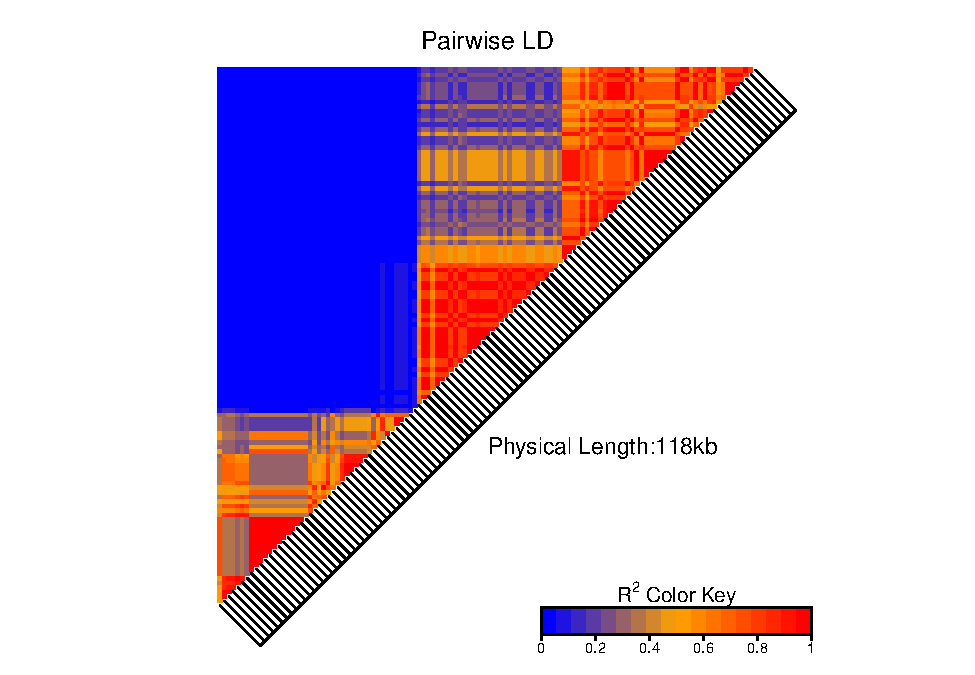
\includegraphics{P032020_LD_files/figure-latex/9th-2.pdf}

We can see that the uncorrelated pairs prevail in the case of the whole
dataset, compared to the case when we filter out the variants with maf
less than 0.35. The argument for that could be that the variants with
maf \textless{} 0.35 don't provide enough ``variation'' in data to show
correlation with other variants.

\begin{enumerate}
\def\labelenumi{\arabic{enumi}.}
\setcounter{enumi}{9}
\tightlist
\item
  (1p) Can you distinguish blocks of correlated markers in the area of
  the FOXP2 gene? How many blocks do you think that \emph{at least} seem
  to exist?
\end{enumerate}

The blocks of correlated markers are more to the red end of the color
spectrum.

For filtered variants there should be at least 2400 pairs which are
correlated (e.g.~R \textgreater{} 0.5). The red triangles divide the
height in roughly 3 parts, and we have 3 halves of a square with side
length of 119/3.

For the original dataset it is hard to get a feeling about the number of
correlated pairs, but a good guess would be to use the same number as
above, i.e.~2400 pairs.

\begin{enumerate}
\def\labelenumi{\arabic{enumi}.}
\setcounter{enumi}{10}
\tightlist
\item
  (1p) Simulate independent SNPs under the assumption of Hardy-Weinberg
  equilibrium, using R's \texttt{sample} instruction
  \texttt{sample(c("AA","AB","BB"),n,replace=TRUE,prob=c(p*p,2*p*q,q*q)))}.
  Simulate as many SNPs as you have in your database, and take care to
  match each SNP in your database with a simulated SNP that has the same
  sample size and allele frequency. Make an LD heatmap of the simulated
  SNPs, using \(R^2\) as your statistic. Compare the results with the LD
  heatmap of the FOXP2 region. What do you observe? State your
  conclusions.
\end{enumerate}

\begin{Shaded}
\begin{Highlighting}[]
\NormalTok{n =}\StringTok{ }\KeywordTok{nrow}\NormalTok{(snp.dataset)}
\NormalTok{sample.snp <-}\StringTok{ }\ControlFlowTok{function}\NormalTok{(x) \{}
\NormalTok{  x.g =}\StringTok{ }\KeywordTok{genotype}\NormalTok{(x, }\DataTypeTok{sep =} \StringTok{"/"}\NormalTok{)}
\NormalTok{  out =}\StringTok{ }\KeywordTok{summary}\NormalTok{(x.g)}
\NormalTok{  p =}\StringTok{ }\NormalTok{out}\OperatorTok{$}\NormalTok{allele.freq[}\DecValTok{1}\NormalTok{,}\DecValTok{2}\NormalTok{]}
\NormalTok{  q =}\StringTok{ }\NormalTok{out}\OperatorTok{$}\NormalTok{allele.freq[}\DecValTok{2}\NormalTok{,}\DecValTok{2}\NormalTok{]}
\NormalTok{  A =}\StringTok{ }\NormalTok{out}\OperatorTok{$}\NormalTok{allele.names[}\DecValTok{1}\NormalTok{]}
\NormalTok{  B =}\StringTok{ }\NormalTok{out}\OperatorTok{$}\NormalTok{allele.names[}\DecValTok{2}\NormalTok{]}
\NormalTok{  AA =}\StringTok{ }\KeywordTok{paste}\NormalTok{(A,A, }\DataTypeTok{sep =} \StringTok{"/"}\NormalTok{)}
\NormalTok{  AB =}\StringTok{ }\KeywordTok{paste}\NormalTok{(A,B, }\DataTypeTok{sep =} \StringTok{"/"}\NormalTok{)}
\NormalTok{  BB =}\StringTok{ }\KeywordTok{paste}\NormalTok{(B,B, }\DataTypeTok{sep =} \StringTok{"/"}\NormalTok{)}
  
  \KeywordTok{return}\NormalTok{(}\KeywordTok{sample}\NormalTok{(}\KeywordTok{c}\NormalTok{(AA,AB,BB),n,}\DataTypeTok{replace=}\OtherTok{TRUE}\NormalTok{,}\DataTypeTok{prob=}\KeywordTok{c}\NormalTok{(p}\OperatorTok{*}\NormalTok{p,}\DecValTok{2}\OperatorTok{*}\NormalTok{p}\OperatorTok{*}\NormalTok{q,q}\OperatorTok{*}\NormalTok{q)))}
\NormalTok{\}}

\NormalTok{sample.dataset =}\StringTok{ }\KeywordTok{data.frame}\NormalTok{(}\KeywordTok{apply}\NormalTok{(snp.dataset, }\DecValTok{2}\NormalTok{, sample.snp))}
\CommentTok{#head(snp.dataset)}
\CommentTok{#head(sample.dataset)}

\NormalTok{RES.sample <-}\StringTok{ }\KeywordTok{data.frame}\NormalTok{(}\KeywordTok{genotype}\NormalTok{(sample.dataset[,}\DecValTok{1}\NormalTok{],}\DataTypeTok{sep=}\StringTok{"/"}\NormalTok{))}

\ControlFlowTok{for}\NormalTok{(i }\ControlFlowTok{in} \DecValTok{2}\OperatorTok{:}\KeywordTok{ncol}\NormalTok{(sample.dataset)) \{}
\NormalTok{   snp <-}\StringTok{ }\KeywordTok{genotype}\NormalTok{(sample.dataset[,i],}\DataTypeTok{sep=}\StringTok{"/"}\NormalTok{)}
\NormalTok{   RES.sample <-}\StringTok{ }\KeywordTok{cbind}\NormalTok{(RES.sample,snp)}
\NormalTok{\}}

\CommentTok{#LDheatmap(RES.sample,LDmeasure="r",color=rgb.palette(18))}

\CommentTok{# We generated the image once but the waiting time was around 10 minutes so we saved the image and present the obtained image so the knitting tool does not need to run LDheatmap again}
\CommentTok{# display image}
\KeywordTok{include_graphics}\NormalTok{(}\StringTok{"./res_sample_heatmap.png"}\NormalTok{, }\DataTypeTok{dpi =} \DecValTok{200}\NormalTok{)}
\end{Highlighting}
\end{Shaded}

\includegraphics[width=7in]{./res_sample_heatmap}

We can see that the generated pairs show almost no correlation when
generated under HW equilibrium assumption, which is very interesting to
see :)

\end{document}
